\documentclass[
%	msc, %% Para dissertações de mestrado, OU
%	mscproposta, %% Para propostas de dissertação de mestrado, OU
	phd, %% Para teses de doutorado, OU
%	phdproposta, %% Para propostas de tese de doutorado
%	portugues %% Para documentos em português, OU
	english %% Para documentos em inglês
]{../ppgccufmg}

%\usepackage[brazil]{babel} %% se o documento for em português, OU
\usepackage[english]{babel} %% se o documento for em inglês
%\usepackage[latin1]{inputenc}
\usepackage{natbib}
\usepackage{xcolor}
\usepackage{lipsum}
\usepackage[
	colorlinks=true,
	linkcolor=blue, %% Cor dos links do sumário
	citecolor=red, %% Cor dos links das citações      
	urlcolor=magenta, %% Cor das urls
]{hyperref}

%% Exemplo 1 de lista customizada: Glossário ==================

\newcommand{\glossario}{
	\chapter*{List of Abbreviations and Acronyms}
	
	\begin{tabular}{ll}
		BFS & \textit{Breadth-First Search}\\
		BOW & \textit{Bag of Words} \\
		TXT & \textit{Text File Format}\\
		UFMG & Universidade Federal de Minas Gerais
	\end{tabular}
}

%% **** Caso não haja nenhuma lista adicional, os comandos acima podem ser apagados. ****
%% ===============================================

%% Exemplo 2 de lista customizada: Lista de algoritmos ==================
%% Para criar uma lista customizada (como Lista de Algoritmos, Lista de Exemplos) que ficará juntamente com as Lista de Figuras e Lista de Tabelas, execute os 3 comandos abaixo substituindo "algoritmos" pelo tipo de lista que estará criando. Para adicionar a lista ao documento, deverá passar o seguinte parâmetro no comando \ppgccufmg:
%% \ppgccufmg{
%% 		...
%% 		listacustomizada={\listadealgoritmos}
%% }
%\newfloat[chapter]{algoritmo}{lol}{Algoritmo}
%\newcommand{\listaalgoritmosname}{Lista de Algoritmos} %% Título da lista
%\newlistof{listadealgoritmos}{lol}{\listaalgoritmosname} %% O primeiro parâmetro é o nome da lista, e este deverá ser passado no parâmetro listacustomizada={\nomedalista}
%\newlistentry{algoritmo}{lol}{0} %% Nome do ambiente de cada algoritmo, e.g., \begin{algoritmo} ... \end{algoritmo}

%% **** Caso não haja nenhuma lista adicional, os comandos acima podem ser apagados. ****
%% ===============================================


\begin{document}
	\ppgccufmg{
		autor={Alan Turing}, %% Autor(a)
		titulo={Systems of Logic Based on Ordinals}, %% Título
		cidade={Belo Horizonte},
		ano={2022},
		versao={Final}, %% Versão do documento
%		orientador={Fulano de tal}, %% Para masculino
		orientadora={Fulana de Tal}, %% Para feminino
%		coorientador={Ciclano}, %% Para masculino
		coorientadora={Ciclana}, %% Para feminino
		fichacatalografica={fichacatalografica.pdf},
		folhadeaprovacao={folhadeaprovacao.pdf},
		resumo={resumo.tex}, %% Resumo em português
		abstracten={abstract.tex}, %% Abstract em inglês
		palavraschave={Matemática. Computação.}, %% Palavras-chave do resumo
		keywords={Math. Computing.}, %% Palavras-chave do abstract
		dedicatoria={dedicatoria.tex}, %% Arquivo .tex contendo a dedicatória
		agradecimentos={agradecimentos.tex},
		epigrafe={Truth and lie are opposite things.},
		epigrafeautor={Unkown},
		listadefiguras={sim}, %% Remova (ou comente) este parâmetro para remover a lista de figuras
		listadetabelas={sim}, %% Remova (ou comente) este parâmetro para remover a lista de tabelas
		listascustomizadas={\glossario} %% Lista customizada (e.g., glossário, lista de algoritmos). 
	}
	
	\chapter{Introdução}
		Exemplo de nota de rodapé \footnote{Aqui está uma nota de rodapé e uma url: \url{https://dcc.ufmg.br}}.
		\lipsum[1-4]
		
		\section{Motivação}
			\lipsum[4-5]
			   
			\subsection{Sub-motivação}
				\lipsum[6-7]
			\subsection{Mais uma sub-motivação}
				\lipsum[8-9]
				\subsubsection{Uma sub-sub-motivação}
					\lipsum[10-11]
	
	\chapter{Desenvolvimento}
		\lipsum[1-4]
		
%		Exemplo de algoritmo ==============================
%		\begin{algoritmo}
%			\centering
%			\framebox[.5\textwidth]{\texttt{Código, Código, Código}}
%			\caption{Este é o meu Algoritmo 1.}
%			\label{alg:algoritmo1}
%		\end{algoritmo}
%	
%		\begin{algoritmo}
%			\centering
%			\framebox[.7\textwidth]{\texttt{Mais Código, Mais Código, Mais Código}}
%			\caption{Este é o meu Algoritmo 2.}
%			\label{alg:algoritmo2}
%		\end{algoritmo}
%		===============================================
		
		\begin{figure}[ht]
			\centering
			\caption{Prédio do DCC em 2016.}
			\label{fig:exemplo}
			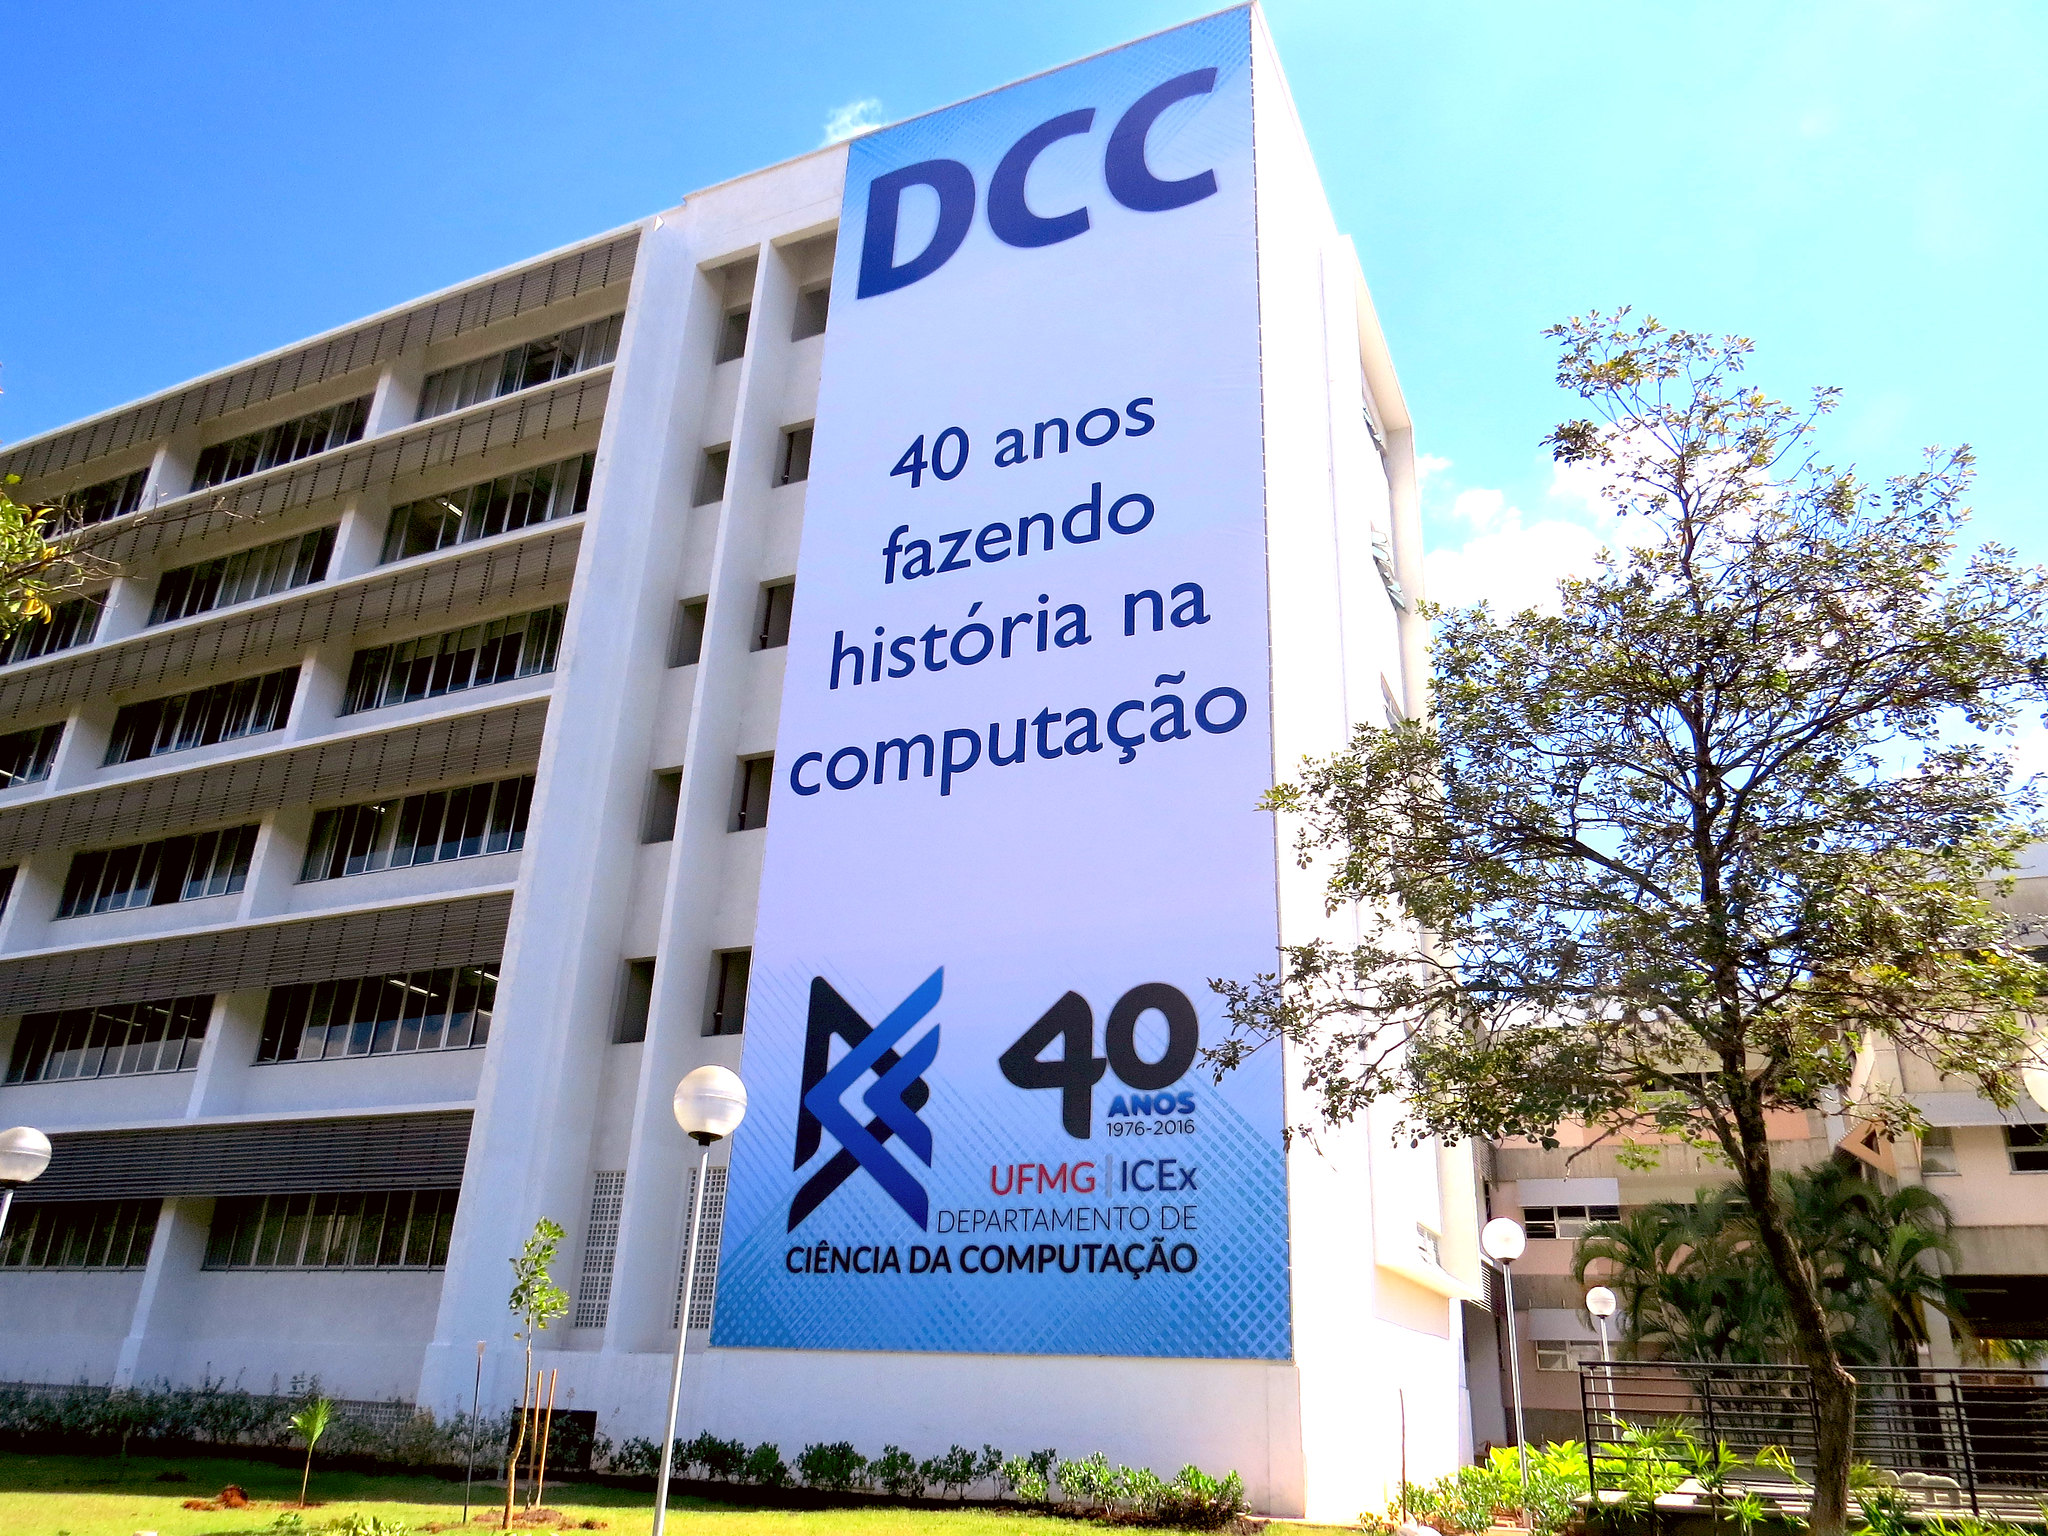
\includegraphics[width=\textwidth]{img/dcc.jpg}
			\small{Fonte:~\url{http://40anos.dcc.ufmg.br/galeria}}
		\end{figure}
	
		\lipsum[5]
		
		\begin{table}[ht]
			\centering
			\begin{tabular}{c|ccccccccl}
				Natural & \multicolumn{9}{c}{Real}   \\ \hline
				1 & 0.  & {\color{red} 2}  & 3   & 6   & 4   & 3   & 6   & 7   & $\ldots$ \\
				2  & 0.  & 0   & {\color{red} 9}  & 8   & 4   & 7   & 3   & 2   & $\ldots$ \\
				3  & 0.  & 1   & 9   & {\color{red} 3}  & 2   & 1   & 4   & 0   & $\ldots$ \\
				4  & 0.  & 8   & 4   & 3   & {\color{red} 2}  & 7   & 9   & 2   & $\ldots$ \\
				5  & 0.  & 0   & 1   & 2   & 9   & {\color{red} 3}  & 4   & 8   & $\ldots$ \\
				6  & 0.  & 2   & 8   & 2   & 6   & 5   & {\color{red} 8}  & 3   & $\ldots$ \\
				7  & 0.  & 0   & 2   & 1   & 5   & 3   & 7   & {\color{red} 4}  & $\ldots$ \\
				$\vdots$ & $\vdots$  & $\vdots$  & $\vdots$  & $\vdots$  & $\vdots$  & $\vdots$  & $\vdots$  & $\vdots$  & $\ddots$ \\ \hline
				\multicolumn{1}{l|}{} & \multicolumn{1}{l}{0.} & \multicolumn{1}{l}{{\color{red} 2}} & \multicolumn{1}{l}{{\color{red} 9}} & \multicolumn{1}{l}{{\color{red} 3}} & \multicolumn{1}{l}{{\color{red} 2}} & \multicolumn{1}{l}{{\color{red} 3}} & \multicolumn{1}{l}{{\color{red} 8}} & \multicolumn{1}{l}{{\color{red} 4}} & $\ldots$
			\end{tabular}
			\caption{Cantor: Existem infinitos diferentes!}
			\label{tab:exemplo}
		\end{table}

		\section{Usando referências}
			Segundo \cite{horn86robot}, todo triângulo equilátero tem os lados iguais. Já segundo \cite{shashua97photometric}, todo quadrado também tem.
			
			Veja que o pacote \verb|natbib| permite uma série de formas diferentes para fazer referências bibliográficas. O comando padrão, \verb|\cite|, realiza a citação comum vista no parágrafo anterior. Outros comandos permitem, por exemplo, colocar automaticamente a citação entre	parênteses \citep{hougen93estimation, sato99illumination2, sato99illumination1, sato01stability}.
			
			O comando usado foi \verb|\citep|. Veja a documentação do \verb|natbib| na Internet para conhecer	outros comandos e exemplos de uso.
			
			Citações aleatórias para fazer com que as referências bibliográficas ocupem	mais de uma página: \cite{bichsel92simple, dror01statistics, guisser92new, dwork2006calibrating, sweeney2002k}.
			
		%% Referências
%		\renewcommand\bibname{Referências} %% Trabalhos em português
		\renewcommand\bibname{References} %% Trabalhos em inglês
		\bibliographystyle{plain}
		\bibliography{referencias}
		
		\begin{apendices}
			\chapter{Um apêndice}
				\lipsum[1-3]
				
			\chapter{Outro Apêndice}
				\lipsum[4-6]
				
		\end{apendices}
		
\end{document}
